\documentclass[11pt]{article}

\usepackage{amsmath}
\usepackage{amssymb}
\usepackage{booktabs}
\usepackage{graphicx}
\usepackage{hyperref}
\usepackage{natbib}
\usepackage[margin=1in]{geometry}
\usepackage{xcolor}
\usepackage{url}
\usepackage[hyphens]{xurl}
\usepackage{pgfplots}
\pgfplotsset{compat=1.17}

\emergencystretch=1em
\sloppy

\hypersetup{
  colorlinks=true,
  linkcolor=blue,
  citecolor=blue,
  urlcolor=blue
}

\title{The Breathing of Groups:\\
Collective Intelligence as an Oscillation Between Coupling and Separation}

\author{
  Philip Phuong Tran\textsuperscript{1}\thanks{Correspondence: Philip Phuong Tran (phil@paragonbiosignals.com)} \\[0.5em]
  \textsuperscript{1} Paragon Biosignals (Univault Technologies LLC), Salt Lake City, Utah, USA
}

\date{}

\begin{document}

\maketitle

\vspace{-1em}

\noindent\textbf{Note on genre and on the companion version.} This is a \emph{theoretical} paper. It introduces no new data. It advances one central claim --- that collective intelligence is maximized by a temporal \emph{rhythm} of coupling and separation rather than by a fixed intermediate coupling --- derives it from a coupled-oscillator model, and states the pre-registered experiment that would confirm or falsify it. It is the dynamic counterpart to a companion static account (``Collective Intelligence Peaks at Partial Synchrony''); the two are offered together so the value of the dynamic proposal can be judged against the simpler static one.

\medskip

\noindent\textbf{Competing Interests:} The author is a co-founder and equity holder of Univault Technologies LLC (d/b/a Paragon Biosignals). This work was funded by Univault Technologies LLC. No new human-subjects data were collected; all empirical results discussed are drawn from the cited published literature.

\bigskip

\begin{abstract}
Human groups solve problems no member can, and a growing literature shows this depends on the coupling between members: too little coupling leaves the group fragmented, too much collapses the independence that collective intelligence requires (groupthink). The standard reading is that group performance is an inverted-U in coupling, maximized at an intermediate value. We argue this static picture is a lower bound on what groups can do, and that the true optimum is \emph{dynamic}. Collective cognition requires two operations with opposite coupling requirements: \emph{sharing} (pooling information, which wants high synchrony) and \emph{generating} (producing novel, non-redundant contributions, which wants independence). No single coupling serves both. A group that \emph{time-multiplexes} --- alternating a coupled phase in which it aligns and pools, and a decoupled phase in which members separate and integrate --- can exceed the performance of any group held at a fixed coupling. We formalize this with a Kuramoto model whose order parameter $r$ is driven between a high and a low value, show that the static functional $\mathrm{CI}(r)\propto r(1-r)$ is the ``do-both-at-once'' bound that time-multiplexing dominates, and predict that the optimum is a limit cycle in $r$ whose period is bounded below by the members' integration timescale. The decoupled phase is where the individual generative act occurs, tying the group rhythm to a within-person integrative state. The framework recovers, and gives a mechanism for, the finding that intermittent breaks in interaction improve collective intelligence. We state three falsifiable predictions and one pre-registered experiment --- that the \emph{temporal pattern} of synchrony predicts group performance beyond its mean --- whose first, cheapest form is a re-analysis of existing data. The account is channel-mediated and near-field; it invokes no physical field, no medium, and no nonlocal term.

\medskip
\noindent\textbf{Keywords:} collective intelligence, coupled oscillators, synchronization, metastability, hyperscanning, intermittent interaction, diversity, groupthink, limit cycle
\end{abstract}

\section{From a fixed optimum to a rhythm}

Groups routinely outperform their members, and the effect tracks the interaction rather than the members' individual ability \citep{woolley2010evidence}. A now-standard account explains why with a tradeoff: collective intelligence needs both integration and independence, so group performance rises and then falls with the strength of coupling between members --- fragmentation when coupling is too weak, groupthink when it is too strong \citep{lorenz2011social, becker2017network}. The performance curve is an inverted-U, and the prescription is to sit at its intermediate peak.

This paper argues that the intermediate peak is a \emph{lower bound}, not the optimum, and that the optimum is a \emph{rhythm}. The intuition is simple and, we will argue, has already been seen without being explained. A group doing real cognitive work must do two incompatible things. It must \emph{share} --- align members' representations and pool what each knows, which is easiest when the group is highly coupled and mutually legible. And it must \emph{generate} --- produce new, non-redundant contributions, which requires members to be independent, precisely the state that coupling destroys. A group frozen at a single intermediate coupling does both operations at once, and does each of them at half strength. A group that \emph{alternates} --- couples to share, separates to generate, then couples again to fold the new contributions in --- can do each operation well in its own phase. Groups, on this view, must \emph{breathe}.

The empirical trace is already on the record: \citet{bernstein2018intermittent} found that groups with \emph{intermittent} breaks in interaction outperform groups in constant interaction, preserving the accuracy of their best members while still improving the average. That is the inverted-U made dynamic, and it is exactly what a breathing group predicts. What has been missing is a mechanism and a measurement, which is what we supply.

\section{The model}

\subsection{Coupled oscillators, coupled by information}

Represent $N$ interacting individuals as phase oscillators, $\theta_i$ with intrinsic frequencies $\omega_i$, evolving under the Kuramoto dynamics \citep{kuramoto1984chemical, strogatz2000kuramoto}
\begin{equation}
\frac{d\theta_i}{dt} = \omega_i + \frac{K(t)}{N}\sum_{j=1}^{N}\sin(\theta_j - \theta_i),
\label{eq:kuramoto}
\end{equation}
with the group state summarized by the order parameter
\begin{equation}
r(t)\,e^{i\psi(t)} = \frac{1}{N}\sum_{j=1}^{N} e^{i\theta_j}, \qquad r \in [0,1].
\label{eq:order}
\end{equation}
As in the companion static account, $K$ is not a physical field coupling but a phenomenological constant standing for the bandwidth and fidelity of information exchange --- language, shared attention, turn-taking, shared representation. The one change here is that we allow $K = K(t)$: the group can modulate how strongly its members are coupled, by choosing to converse or to work apart, and $r(t)$ follows. Neural and physiological rhythms are entrainable and phase-align during interaction to a degree that tracks its quality \citep{stephens2010speaker, dikker2017brain}; that the brain's own coordination is \emph{metastable}, continually forming and dissolving synchrony rather than locking, is itself well documented \citep{tognoli2014metastable}, and is the within-person analogue of the group rhythm we propose.

For heterogeneity of half-width $\gamma$ (viewpoint diversity) with a Lorentzian $g(\omega)$, synchronization onsets at $K_c = 2\gamma$ \citep{acebron2005kuramoto}, so more diverse groups require stronger coupling to cohere; near onset $r \sim \sqrt{K-K_c}$ \citep{strogatz2000kuramoto}. These fix the two coupling levels the rhythm will move between. (Eq.~\eqref{eq:kuramoto} is mean-field; on a network $K_c \propto 1/\lambda_{\max}(A)$ \citep{restrepo2005onset}, and finite $N$ rounds the transition --- see Section~\ref{sec:scope}.)

\subsection{The static bound}

Collective intelligence is not synchrony. Integration is captured by $r$; retained independence is captured by the dispersion of the phase distribution, and by the exact identity of directional statistics the circular variance is $1-r$ \citep{mardia2000directional}. To leading order,
\begin{equation}
\mathrm{CI}_{\text{static}}(r) \;\propto\; \underbrace{r}_{\text{integration}}\,\underbrace{(1-r)}_{\text{retained independence}},
\label{eq:static}
\end{equation}
which is unimodal, peaking at partial synchrony (the companion paper develops this case). Equation~\eqref{eq:static} is the performance of a group that does sharing and generating \emph{simultaneously}, at one value of $r$: it is the ``do-both-at-once'' bound, and it is capped (the symmetric form at $r=1/2$ gives $\mathrm{CI}\le 1/4$).

\subsection{The dynamic claim}

Now separate the two operations in time. Let sharing accrue value at a rate $S(r)$ that increases with synchrony (aligning and pooling is easier when the group is coupled), and let generating accrue value at a rate $G(r)$ that increases with independence (novel, non-redundant contributions require members to differ). A group that spends a fraction of each cycle near a high level $r_{\uparrow}$ and the remainder near a low level $r_{\downarrow}$ produces, per cycle, a collective yield of the schematic form
\begin{equation}
Y_{\text{cycle}} \;\propto\; S(r_{\uparrow})\cdot G(r_{\downarrow}) \;-\; C_{\text{switch}},
\label{eq:cycle}
\end{equation}
where $C_{\text{switch}}$ is the cost of transitioning between phases. The essential point is comparative: because $S$ and $G$ are maximized at \emph{opposite} ends of $r$, the product $S(r_{\uparrow})G(r_{\downarrow})$ with $r_{\uparrow}\to 1$, $r_{\downarrow}\to 0$ can exceed $S(\bar r)G(\bar r)$ at any single intermediate $\bar r$, provided the switching cost is smaller than the gain. When it is, the time-averaged performance of a \emph{breathing} group dominates the static optimum of Eq.~\eqref{eq:static}, and the optimal trajectory of $r(t)$ is a \emph{limit cycle}, not a fixed point (Fig.~\ref{fig:breathe}).

We are careful about what this is. We do not prove a general dominance theorem; Eq.~\eqref{eq:cycle} is an illustrative functional, and the dominance holds under stated conditions --- that sharing and generating are genuinely separable in time, that their value multiplies rather than merely adds, and that switching is cheap relative to the benefit. Whether real groups satisfy these conditions is the empirical question, and \citet{bernstein2018intermittent} is existing evidence that at least some do. The claim we defend is structural: \emph{when two complementary operations have opposing coupling requirements, time-multiplexing beats any static compromise, and the optimum is dynamic.}

\begin{figure}[ht]
\centering
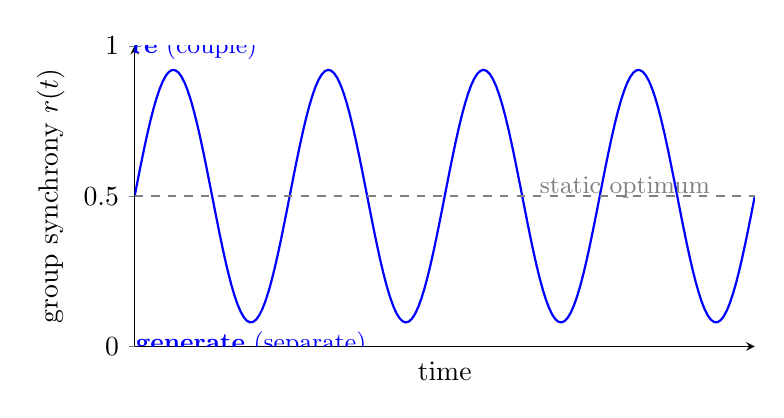
\begin{tikzpicture}
\begin{axis}[
  width=0.78\textwidth, height=5.4cm,
  xlabel={time}, ylabel={group synchrony $r(t)$},
  xmin=0, xmax=4, ymin=0, ymax=1,
  samples=200, domain=0:4,
  axis lines=left, ytick={0,0.5,1}, xtick=\empty,
  every axis plot/.append style={thick}
]
\addplot[blue, thick] {0.5 + 0.42*sin(deg(2*pi*x))};
\addplot[gray, dashed] {0.5};
\node[anchor=south, blue] at (axis cs:0.25,0.92) {\small \textbf{share} (couple)};
\node[anchor=north, blue] at (axis cs:0.75,0.08) {\small \textbf{generate} (separate)};
\node[anchor=west, gray] at (axis cs:2.55,0.53) {\small static optimum};
\end{axis}
\end{tikzpicture}
\caption{Collective intelligence as a rhythm. A group that holds a fixed intermediate synchrony (gray dashed) does sharing and generating simultaneously and at half strength. A \emph{breathing} group (blue) alternates a coupled phase in which it aligns and pools information (high $r$) with a decoupled phase in which members separate and produce novel contributions (low $r$). When sharing and generating are maximized at opposite ends of $r$, the breathing trajectory's time-averaged performance exceeds the static optimum. The optimum is a limit cycle in $r$, not a fixed point.}
\label{fig:breathe}
\end{figure}

\subsection{Tempo: why the period cannot be arbitrarily fast}

The decoupled phase is not empty time; it is when generating happens. A member separated from the group integrates what was pooled and produces a candidate contribution, and integration takes time --- a characteristic timescale $\tau_{\text{int}}$. If the group re-couples before $\tau_{\text{int}}$ has elapsed, the decoupled phase yields no new writes and the breath is wasted. The optimal period $T^\ast$ is therefore bounded below by the members' integration timescale,
\begin{equation}
T^\ast \gtrsim \tau_{\text{int}},
\end{equation}
and there is a matching upper bound set by forgetting and drift (separate too long and the shared context decays). This predicts a \emph{finite optimal tempo}, tied to a measurable within-person quantity, and it explains why constant interaction ($T\to 0$) underperforms \citep{bernstein2018intermittent}: it never allows a full generative breath.

\section{The generative phase, at the level of the person}

The group's decoupled phase corresponds to a specific individual state, and this ties the macroscopic rhythm to within-person neuroscience without invoking anything exotic. Producing a novel contribution --- the ``write'' that charges the group's shared pool --- is associated with quieting the effortful, self-referential foreground: down-regulation of the default-mode network and the narrative self allows previously backgrounded associations to surface \citep{brewer2011meditation}. This is the same integrative mode the brain enters when external input is gated and it consolidates and recombines the day's information. In the breathing picture, the group's low-$r$ phase is the collective invitation for each member to enter that generative, integrative state; the high-$r$ phase re-couples members so the products can be shared and aligned. The rhythm is thus doubly grounded: it is a limit cycle in the group order parameter and a cycle between coupled sharing and decoupled integration in the individual.

\section{Predictions and the decisive experiment}
\label{sec:exp}

The framework's core prediction is that the \emph{temporal structure} of synchrony, not merely its average, governs group performance. We state three consequences, each with its refutation, and one pre-registered study.

\begin{enumerate}
  \item \textbf{Rhythm beats stasis.} Group performance depends on the temporal pattern of $r(t)$ beyond its time-average. Groups whose synchrony \emph{alternates} between high and low values outperform groups held at any fixed $r$, including the static optimum. \emph{Refuted if}: performance is fully explained by mean $r$, with no added variance from its temporal dynamics.
  \item \textbf{The write lives in the trough.} High-value contributions --- those that most improve the collective solution --- are produced during an individual's decoupled, integrative state (a momentary drop in that member's coupling to the group, with the corresponding within-person integrative signature), not during high coupling. \emph{Refuted if}: contribution value is uncorrelated with the writer's momentary coupling and internal state.
  \item \textbf{Tempo matching.} The performance-maximizing alternation period is finite and scales with the members' integration timescale $\tau_{\text{int}}$; both too-fast and too-slow alternation underperform. \emph{Refuted if}: performance is flat in, or monotone in, alternation period.
\end{enumerate}

\paragraph{The pre-registered experiment.} Small groups solve a series of problems that require both pooling and independent insight, under continuous hyperscanning (EEG/physiology) of all members. We compute time-resolved inter-brain synchrony $r(t)$, each member's momentary decoupling and internal integrative state, and the value of each contribution to the evolving collective solution. The confirmatory, pre-registered test of Prediction~1 specifies \emph{in advance} that a model using the temporal dynamics of $r(t)$ (e.g.\ its alternation amplitude and period) predicts group performance significantly beyond a model using mean $r$ alone; the framework is falsified if the temporal term adds nothing.

\paragraph{Controls and standards.} The load-bearing control is a \textbf{surrogate-pair (pseudo-hyperscanning) null}: because two people attending to the same stimulus will show correlated, even lagged and asymmetric, activity with no interaction-specific coupling, every coupling estimate must exceed a partner-shuffled distribution before it is interpreted \citep{burgess2013conceptual, novembre2021hyperscanning, hamilton2021hyperscanning}. Coupling is estimated with standard, reproducible measures --- phase-locking value, the imaginary part of coherency to suppress volume-conduction artifacts \citep{nolte2004identifying}, transfer entropy \citep{schreiber2000measuring}, convergent cross-mapping \citep{sugihara2012detecting}. Protocols and analysis plans are pre-registered; analysts are blinded; inference uses permutation and cluster-based methods with multiple-comparison correction and reported effect sizes; independent replication is required.

\paragraph{The cheapest first test.} No new data are needed to begin. \citet{bernstein2018intermittent} and open hyperscanning datasets with performance measures \citep{dikker2017brain} already contain the temporal structure of interaction. A re-analysis asking whether the \emph{alternation} of interaction (or of measured synchrony), with an a-priori tempo dependence, predicts performance beyond its mean is a direct, low-cost test of Prediction~1 and Prediction~3.

\section{Relation to known results}

The static inverted-U --- fragmentation at low coupling, groupthink at high --- is well established \citep{lorenz2011social, becker2017network, lazer2007network}; we treat it as the simultaneous, do-both-at-once bound. The dynamic improvement is likewise not invented here: \citet{bernstein2018intermittent} demonstrated it behaviorally, and metastable coordination dynamics \citep{tognoli2014metastable} show the same couple-and-release rhythm inside a single brain. Our contribution is to unify these under one order-parameter model, to give the rhythm a mechanism (complementary operations with opposing coupling requirements), and to make it quantitative and falsifiable: a finite optimal tempo tied to $\tau_{\text{int}}$, and a performance dependence on the temporal pattern of $r$ that a pre-registered study can confirm or kill.

\section{Scope, boundary, and limits}
\label{sec:scope}

The framework is bounded exactly as its static companion is: coupling is informational and near-field, correlations are distance-dependent and decay with channel degradation, and there is no nonlocal correlation and no physical medium.\footnote{An earlier formulation by the author proposed a planetary (geomagnetic / Schumann-band) medium mediating inter-individual coupling; that claim is withdrawn on physical grounds (a warm biological source cannot drive a planetary cavity mode above the lightning-driven background, and body-temperature scales forbid the required persistent coherence) and plays no role here. The word ``coherence'' is retained only in its measurable sense: phase alignment between oscillators.} Two internal limits are stated plainly. \textbf{Finite $N$}: the transition and $K_c=2\gamma$ are $N\to\infty$ results; real groups have $N\sim 2$--$10$, where $r$ fluctuates at order $1/\sqrt N$ and the ``limit cycle'' is a noisy quasi-periodic alternation rather than a clean orbit --- the predictions are correspondingly about statistical tendencies, not deterministic curves. \textbf{Topology}: Eq.~\eqref{eq:kuramoto} is all-to-all; a network model with directed coupling ($K_c$ set by $\lambda_{\max}$ \citep{restrepo2005onset}) is the honest next step and connects the rhythm to the structure literature \citep{lazer2007network, becker2017network}. Finally, the schematic yield of Eq.~\eqref{eq:cycle} should be replaced, in future work, by a functional derived from the phase-density dynamics (e.g.\ via the Ott--Antonsen reduction \citep{ott2008low}) so that the optimal duty cycle and tempo are computed rather than posited.

\section{Conclusion}

The lesson of the collective-intelligence literature is usually stated as a set-point: keep a group at intermediate coupling. We argue the truer lesson is a rhythm: a group must \emph{breathe} --- couple to share, separate to generate, couple again to fold the new in --- because sharing and generating pull the group toward opposite ends of synchrony and cannot both be served at once. The static inverted-U is the price of trying; the breath is how a group stops paying it. The claim is modest in what it assumes --- a coupled-oscillator model, a circular-variance identity, and an already-observed benefit of intermittent interaction --- and precise in what it risks: a finite optimal tempo tied to the members' integration timescale, and a group performance that depends on the temporal pattern of synchrony beyond its mean. Both are measurable, and the first can be tested on data that already exist. If groups do not breathe, this is wrong, and a single pre-registered re-analysis can say so.

\bigskip

\noindent\textbf{Data and code availability.} This is a theoretical paper; it generates no new data. The figure is produced by the plotted equations and requires no data.

\bigskip

\bibliographystyle{plainnat}

\begin{thebibliography}{99}

\bibitem[Acebr{\'o}n et~al.(2005)]{acebron2005kuramoto}
J.~A.~Acebr{\'o}n, L.~L.~Bonilla, C.~J.~P{\'e}rez~Vicente, F.~Ritort, and R.~Spigler.
\newblock The Kuramoto model: A simple paradigm for synchronization phenomena.
\newblock \emph{Reviews of Modern Physics}, 77(1):137--185, 2005.

\bibitem[Becker et~al.(2017)]{becker2017network}
J.~Becker, D.~Brackbill, and D.~Centola.
\newblock Network dynamics of social influence in the wisdom of crowds.
\newblock \emph{Proceedings of the National Academy of Sciences}, 114(26):E5070--E5076, 2017.

\bibitem[Bernstein et~al.(2018)]{bernstein2018intermittent}
E.~Bernstein, J.~Shore, and D.~Lazer.
\newblock How intermittent breaks in interaction improve collective intelligence.
\newblock \emph{Proceedings of the National Academy of Sciences}, 115(35):8734--8739, 2018.

\bibitem[Brewer et~al.(2011)]{brewer2011meditation}
J.~A.~Brewer, P.~D.~Worhunsky, J.~R.~Gray, Y.~Y.~Tang, J.~Weber, and H.~Kober.
\newblock Meditation experience is associated with differences in default mode network activity and connectivity.
\newblock \emph{Proceedings of the National Academy of Sciences}, 108(50):20254--20259, 2011.

\bibitem[Burgess(2013)]{burgess2013conceptual}
A.~P.~Burgess.
\newblock On the interpretation of synchronization in EEG hyperscanning studies: a cautionary note.
\newblock \emph{Frontiers in Human Neuroscience}, 7:881, 2013.

\bibitem[Dikker et~al.(2017)]{dikker2017brain}
S.~Dikker, L.~Wan, I.~Davidesco, L.~Kaggen, M.~Oostrik, J.~McClintock, J.~Rowland, G.~Michalareas, J.~J.~Van~Bavel, M.~Ding, and D.~Poeppel.
\newblock Brain-to-brain synchrony tracks real-world dynamic group interactions in the classroom.
\newblock \emph{Current Biology}, 27(9):1375--1380, 2017.

\bibitem[Hamilton(2021)]{hamilton2021hyperscanning}
A.~F.~de~C.~Hamilton.
\newblock Hyperscanning: Beyond the hype.
\newblock \emph{Neuron}, 109(3):404--407, 2021.

\bibitem[Kuramoto(1984)]{kuramoto1984chemical}
Y.~Kuramoto.
\newblock \emph{Chemical Oscillations, Waves, and Turbulence}.
\newblock Springer, Berlin, 1984.

\bibitem[Lazer and Friedman(2007)]{lazer2007network}
D.~Lazer and A.~Friedman.
\newblock The network structure of exploration and exploitation.
\newblock \emph{Administrative Science Quarterly}, 52(4):667--694, 2007.

\bibitem[Lorenz et~al.(2011)]{lorenz2011social}
J.~Lorenz, H.~Rauhut, F.~Schweitzer, and D.~Helbing.
\newblock How social influence can undermine the wisdom of crowd effect.
\newblock \emph{Proceedings of the National Academy of Sciences}, 108(22):9020--9025, 2011.

\bibitem[Mardia and Jupp(2000)]{mardia2000directional}
K.~V.~Mardia and P.~E.~Jupp.
\newblock \emph{Directional Statistics}.
\newblock Wiley, Chichester, 2000.

\bibitem[Nolte et~al.(2004)]{nolte2004identifying}
G.~Nolte, O.~Bai, L.~Wheaton, Z.~Mari, S.~Vorbach, and M.~Hallett.
\newblock Identifying true brain interaction from EEG data using the imaginary part of coherency.
\newblock \emph{Clinical Neurophysiology}, 115(10):2292--2307, 2004.

\bibitem[Novembre and Iannetti(2021)]{novembre2021hyperscanning}
G.~Novembre and G.~D.~Iannetti.
\newblock Hyperscanning alone cannot prove causality. Multibrain stimulation can.
\newblock \emph{Trends in Cognitive Sciences}, 25(2):96--99, 2021.

\bibitem[Ott and Antonsen(2008)]{ott2008low}
E.~Ott and T.~M.~Antonsen.
\newblock Low dimensional behavior of large systems of globally coupled oscillators.
\newblock \emph{Chaos}, 18(3):037113, 2008.

\bibitem[Restrepo et~al.(2005)]{restrepo2005onset}
J.~G.~Restrepo, E.~Ott, and B.~R.~Hunt.
\newblock Onset of synchronization in large networks of coupled oscillators.
\newblock \emph{Physical Review E}, 71(3):036151, 2005.

\bibitem[Schreiber(2000)]{schreiber2000measuring}
T.~Schreiber.
\newblock Measuring information transfer.
\newblock \emph{Physical Review Letters}, 85(2):461--464, 2000.

\bibitem[Stephens et~al.(2010)]{stephens2010speaker}
G.~J.~Stephens, L.~J.~Silbert, and U.~Hasson.
\newblock Speaker--listener neural coupling underlies successful communication.
\newblock \emph{Proceedings of the National Academy of Sciences}, 107(32):14425--14430, 2010.

\bibitem[Strogatz(2000)]{strogatz2000kuramoto}
S.~H.~Strogatz.
\newblock From Kuramoto to Crawford: exploring the onset of synchronization in populations of coupled oscillators.
\newblock \emph{Physica D}, 143(1--4):1--20, 2000.

\bibitem[Sugihara et~al.(2012)]{sugihara2012detecting}
G.~Sugihara, R.~May, H.~Ye, C.~H.~Hsieh, E.~Deyle, M.~Fogarty, and S.~Munch.
\newblock Detecting causality in complex ecosystems.
\newblock \emph{Science}, 338(6106):496--500, 2012.

\bibitem[Tognoli and Kelso(2014)]{tognoli2014metastable}
E.~Tognoli and J.~A.~S.~Kelso.
\newblock The metastable brain.
\newblock \emph{Neuron}, 81(1):35--48, 2014.

\bibitem[Woolley et~al.(2010)]{woolley2010evidence}
A.~W.~Woolley, C.~F.~Chabris, A.~Pentland, N.~Hashmi, and T.~W.~Malone.
\newblock Evidence for a collective intelligence factor in the performance of human groups.
\newblock \emph{Science}, 330(6004):686--688, 2010.

\end{thebibliography}

\end{document}
